\section{1174057 Alit Fajar Kurniawan}

\subsection{Teori}
\begin{enumerate}
\item Jelaskan apa itu random forest, sertakan gambar ilustrasi buatan sendiri.
\par
Random Forest merupakan algoritma yang digunakan terhadapap klasifikasi data dalam jumlah yang besar. Klasifikasi pada random forest dilakukan dengan penggabungan dicision tree dengan melakuakn training terhadap sempel data yang dimiliki. Semakin banyak dicision tree maka data yang di dapat akan semakin akurat. Dibawah ini merupakan salah satu ilustrasi penggunaan Random Forest..

\begin{figure}[ht]
\centering
\includegraphics[scale=0.5]{figures/1174057/chapter3/1.png}
\caption{Random Forest}
\label{contoh}
\end{figure}


\item Jelaskan cara membaca dataset khusus dan artikan makna setiap file dan isi field masing masing file \par Pertama download dataset terlebih dahulu lalu buka dengan menggunakan software spyder guna melihat isi dari dataset tersebut. Data tersebut memiliki extensi file bernama .txt dan didalamnya terdapat class dari field. Misalnya saja pada data jenis burung memiliki file index dan angka, dimana index berisi angka yang memiliki makna berupa jenis burung atau bahkan nama burung sedangkan field memiliki isi nilai berupa 0 dan 1 yang dimana sifatnya boolean atau Ya dan Tidak. Hal ini dikarenakan komputer hanya dapat membaca bilangan biner maka dari itu field yang di isikan berupa angka. Artinya angka 0 berarti tidak dan angka 1 berarti Ya.

\item Jelaskan apa itu Cross Validation 
\par 
Cross Validation merupakan sebuah teknik validasi model yang digunakan untuk menilai bagaimana hasil analisis statistik akan digeneralisasi ke kumpulan data independen. Cross validation digunakan dengan tujuan prediksi, dan bila kita ingin memperkirakan seberapa akurat model model prediksi yang dilakukan dalam sebuah praktek. Tujuan dari cross validation yaitu untuk mendefinisikan dataset guna menguju dalam fase pelatihan untuk membatasi masalah seperti overfitting dan underfitting serta mendapatkan wawasan tentang bagaimana model akan digeneralisasikan ke set data independen.

\item Jelaskan apa arti score 44 \% pada random forest, 27 \% pada decision tree dan 29 \% dari SVM \par Dimana Score 44 \% diperoleh dari hasil pengelohan dataset jenis burung. Dimana akan dilakukan proses pembagian data testing dan data training lalu diproses dan menghasilkan score sebanyak 44 \% dimana menjelaskan bahwa score tersebut digunakan sebagai pembanding dalam tingkat keakuratannya. Pada dicision tree akan memperoleh data lebih kecil yaitu sebanyak 27 \% hal ini dikarenakan data yang diolah menggunakan dicision tree dibagi menjadi beberapa tree dan lalu disimpulkan untuk mendapatkan data yang akurat. Pada SVM akan memperoleh score sebanyak 29 \% hal ini dikarenakan data yang dimiliki masih bernilai netral sehingga tingkat keakuratannya masih belum jelas.

\item Jelaskan bagaimana cara membaca confusion matriks dan contohnya memakai gambar atau ilustrasi sendiri.
Untuk membaca confusion matriks dapat menggunakan source code sebagai berikut,
	\begin{verbatim}
		import numpy as np
		np.set_printoptions(precision=2)
		plt.figure(figsize=(60,60), dpi=300)
		plot_confusion_matrix(cm, classes=birds, normalize=True)
		plt.show()
	\end{verbatim}

Dimana numpy akan mengurus semua data yang berhubungan dengan matrix. Pada source code tersebut digunakan dalam melakukan read pada dataset burung dengan menggunakan metode confusion matrix. Dalam confusion matrix memiliki 4 istilah yaitu True Positive yang merupakan data posotif yang terditeksi benar, True Negatif yang merupakan data negatif akan tetapi terditeksi benar, False Positif merupakan data negatif namun terditeksi sebagai data positif, False Negatif merupakan data posotif namun terditeksi sebagai data negatif. Adapun contoh hasil read dataset menggunakan confusion matrix dapat dilihat pada figure \ref{YNCM}
	
	\begin{figure}[ht]
	\centerline{\includegraphics[scale=0.5]{figures/1174057/chapter3/2.PNG}}
	\caption{Confusion Matrix.}
	\label{YNCM}
	\end{figure}

\item Jelaskan apa itu voting pada random forest disertai dengan ilustrasi gambar sendiri.\par
Voting merupakan proses pemilihan dari tree yang dimana akan dimunculkan hasilnya dan disimpulkan menjadi informasi yang pasti. Untuk kebih jelasnya saya akan memberikan sebuah contoh bagaimana voting bekerja.
	
	\begin{figure}[ht]
	\centerline{\includegraphics[width=1\textwidth]{figures/1174057/chapter3/3.PNG}}
	\caption{Voting.}
	\label{gambar}
	\end{figure}

Dimana ditunjukkan pada figure \ref{YNV} terdapat 3 tree. Dalam tree tersebut akan dilakukan proses voting. Saya akan memberikan contoh kasus, dimana akan diadakan voting untuk menentukan sebuah mobil. Dalam tree akan diberikan sejumlah data misalnya saja data tersebut berupa gambar, yang dimana data tersebut akan dipilih dengan cara voting. Hasil voting akhir dari setiap tree menunjukkan mobil jazz, yang berarti kesimpulan dari data yang telah diberikan menyatakan gambar tersebut adalah mobil jazz. Bagaimana apabila terjadi perbedaan data misalnya saja pada tree 1 dan 2 menunyatakan mobil jazz sedangkan pada tree 3 menyatakan mobil yaris, maka kesimpulan yang di ambil adalah mobil jazz dikarenakan hasil voting terbanyak adalah mobil jazz.
\end{enumerate}


\subsection{Praktikum}
\begin{enumerate}
\item pandas \par
pada baris ke satu yaitu perintah mengimport library padas pada python atau anaconda kemudian di inisialisasikan menjadi karakter. selanjutnya ada sebuah array yang berisi nama cewek. selanjutnya penggunaan array tipe series dan yang terakhir perintah print untuk menampilkan data pada karakter \ref{contoh1}.
\lstinputlisting{src/1174057/chapter3/1.py}
\begin{figure}[ht]
\centering
\includegraphics[scale=1]{figures/1174057/chapter3/4.PNG}
\caption{hasil}
\label{contoh1}
\end{figure}

\item numpy\par
Source Code baris pertama menjelaskan akan melakukan import pada library numpy dan di rename dengan alit. Selanjutnya kita akan membuat matrix dengan numpy dengan menggunakan fungsi eye. baris kedua selanjutnya kita akan memanggil matrix identitas 10x10. Fungsi eye disini berguna untuk memanggil matrix identitas dengan jumlah colom dan baris sesuai yang ditentukan. Disini saya telah menentukan 10 colom dan baris maka dari itu hasilnya akan memunculkan matrix identitas 10x10, untuk lebih jelasnya dapat dilihat pada fugure \ref{contoh2}
\lstinputlisting{src/1174057/chapter3/2.py}
\begin{figure}[ht]
\centering
\includegraphics[scale=0.7]{figures/1174057/chapter3/5.PNG}
\caption{hasil}
\label{contoh2}
\end{figure}

\item matplotlib\par
Arti tiap baris aplikasi sederhana matplotlib item Pada baris pertama akan melakukan import library Matplotlib dan di rename menjadi fajar. Pada baris kedua kita akan memberikan nilai plot atau grafik  pada library fajar. Pada baris ketiga kita akan memberikan nama atau label pada grafik tersebut. Pada baris terakhir kita akan melakukan show sehingga grafik dapat kita lihat. Jalankan source code diatas dengan spyder sehingga hasilnya akan nampak seperti pada figure \ref{contoh3}
\lstinputlisting{src/1174057/chapter3/3.py}
\begin{figure}[ht]
\centering
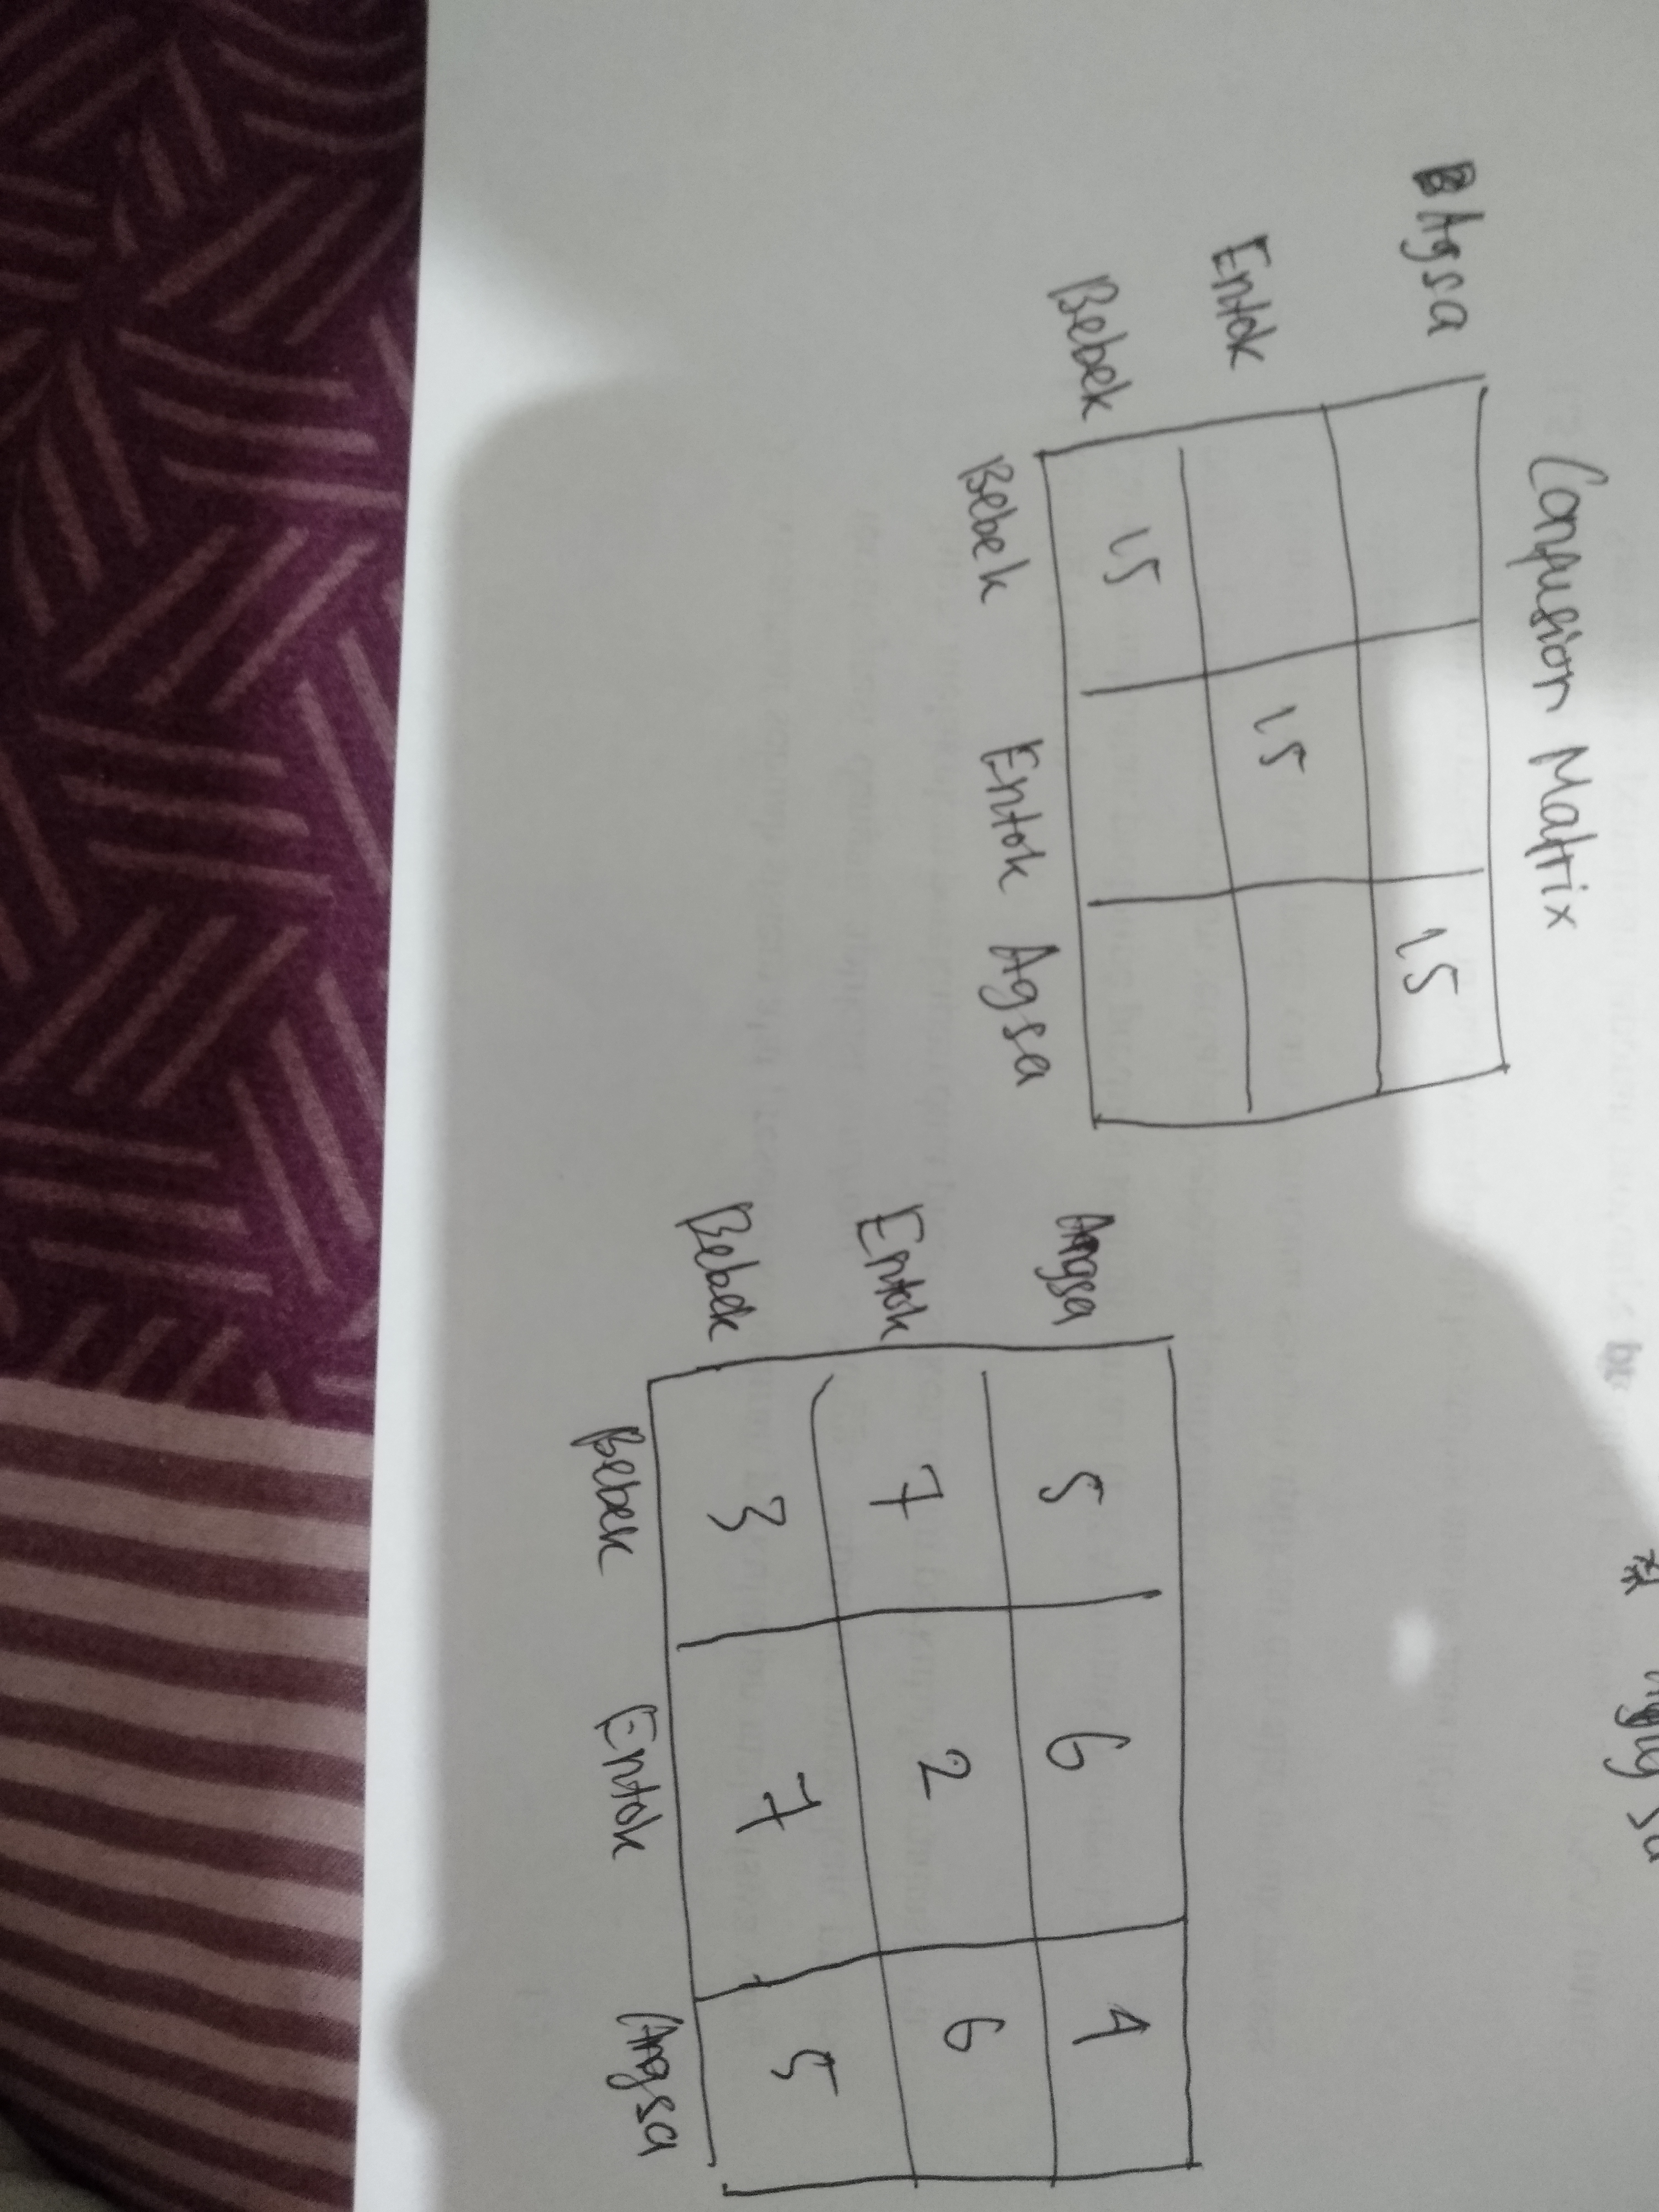
\includegraphics[scale=0.5]{figures/1174057/chapter3/6.PNG}
\caption{hasil}
\label{contoh3}
\end{figure}

\subitem Selanjutnya perhatikan source code berikut ini,
\lstinputlisting{src/1174057/chapter3/4.py}
Pada baris pertama akan melakukan import library Matplotlib dan di rename menjadi alit. Pada baris kedua dan ketiga kita akan menentukan nilai pada variabel a dan f.Pada baris keempat kita akan membuat diagram batang dengan fungsi bar. Pada baris kelima kita akan memberikan nama atau label pada diagram batang tersebut. Pada baris terakhir kita akan melakukan show sehingga kita dapat melihat hasilnya. Jalankan source code tersebut di dalam spyder maka hasilnya akan nampak seperti pada figure \ref{contohlagi}
	
\begin{figure}[ht]
\centerline{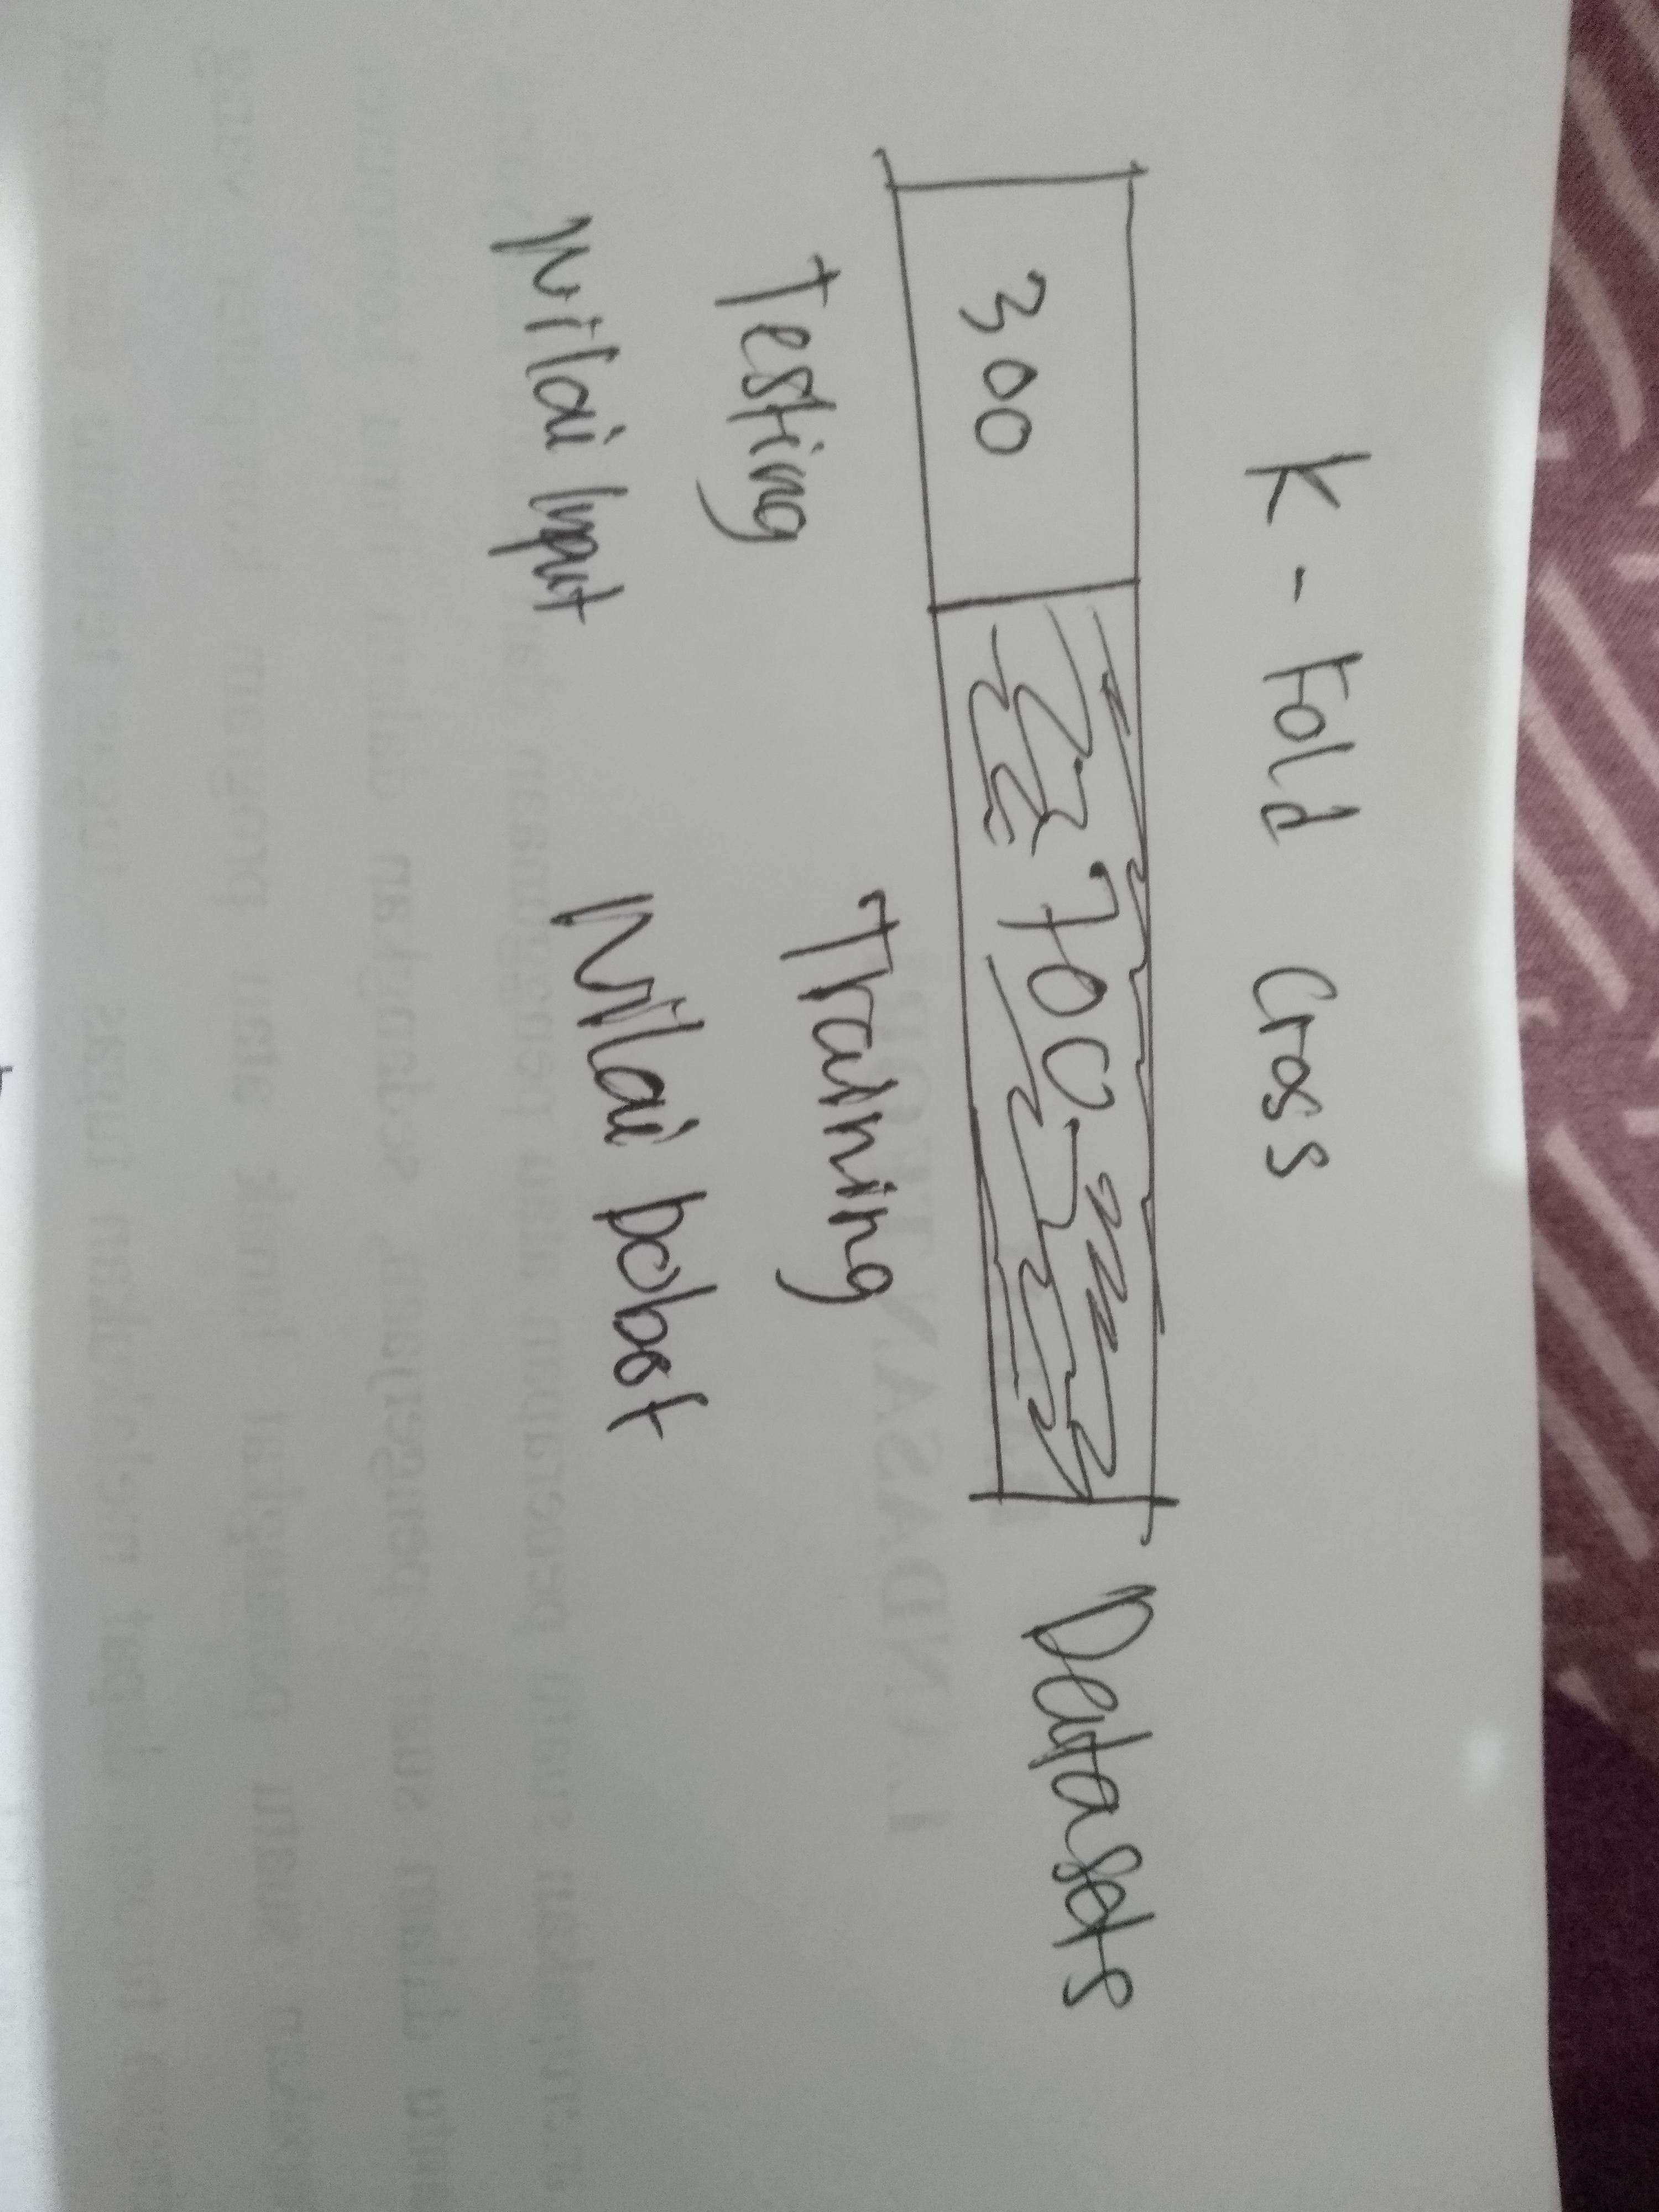
\includegraphics[width=1\textwidth]{figures/1174057/chapter3/7.PNG}}
\caption{Aplikasi Sederhana Dengan Matplotlib Diagram Batang.}
\label{contohlagi}
\end{figure}

\item Random Forest\par
Arti tiap baris hasil codingan random forest pada baris pertama random forest di import dari sklearn dengan ketentuan yaitu Nilai default untuk parameter yang mengontrol ukuran pohon (mis. Max\_depth, min\_samples\_leaf, dll.) Mengarah ke pohon yang tumbuh besar dan tidak di-unsuned yang berpotensi sangat besar pada beberapa set data. Untuk mengurangi konsumsi memori, kompleksitas dan ukuran pohon harus dikontrol dengan menetapkan nilai parameter tersebut. hasil pada gambar \ref{contoh4} . 
\lstinputlisting{src/1174057/chapter3/5.py}
\begin{figure}[ht]
\centering
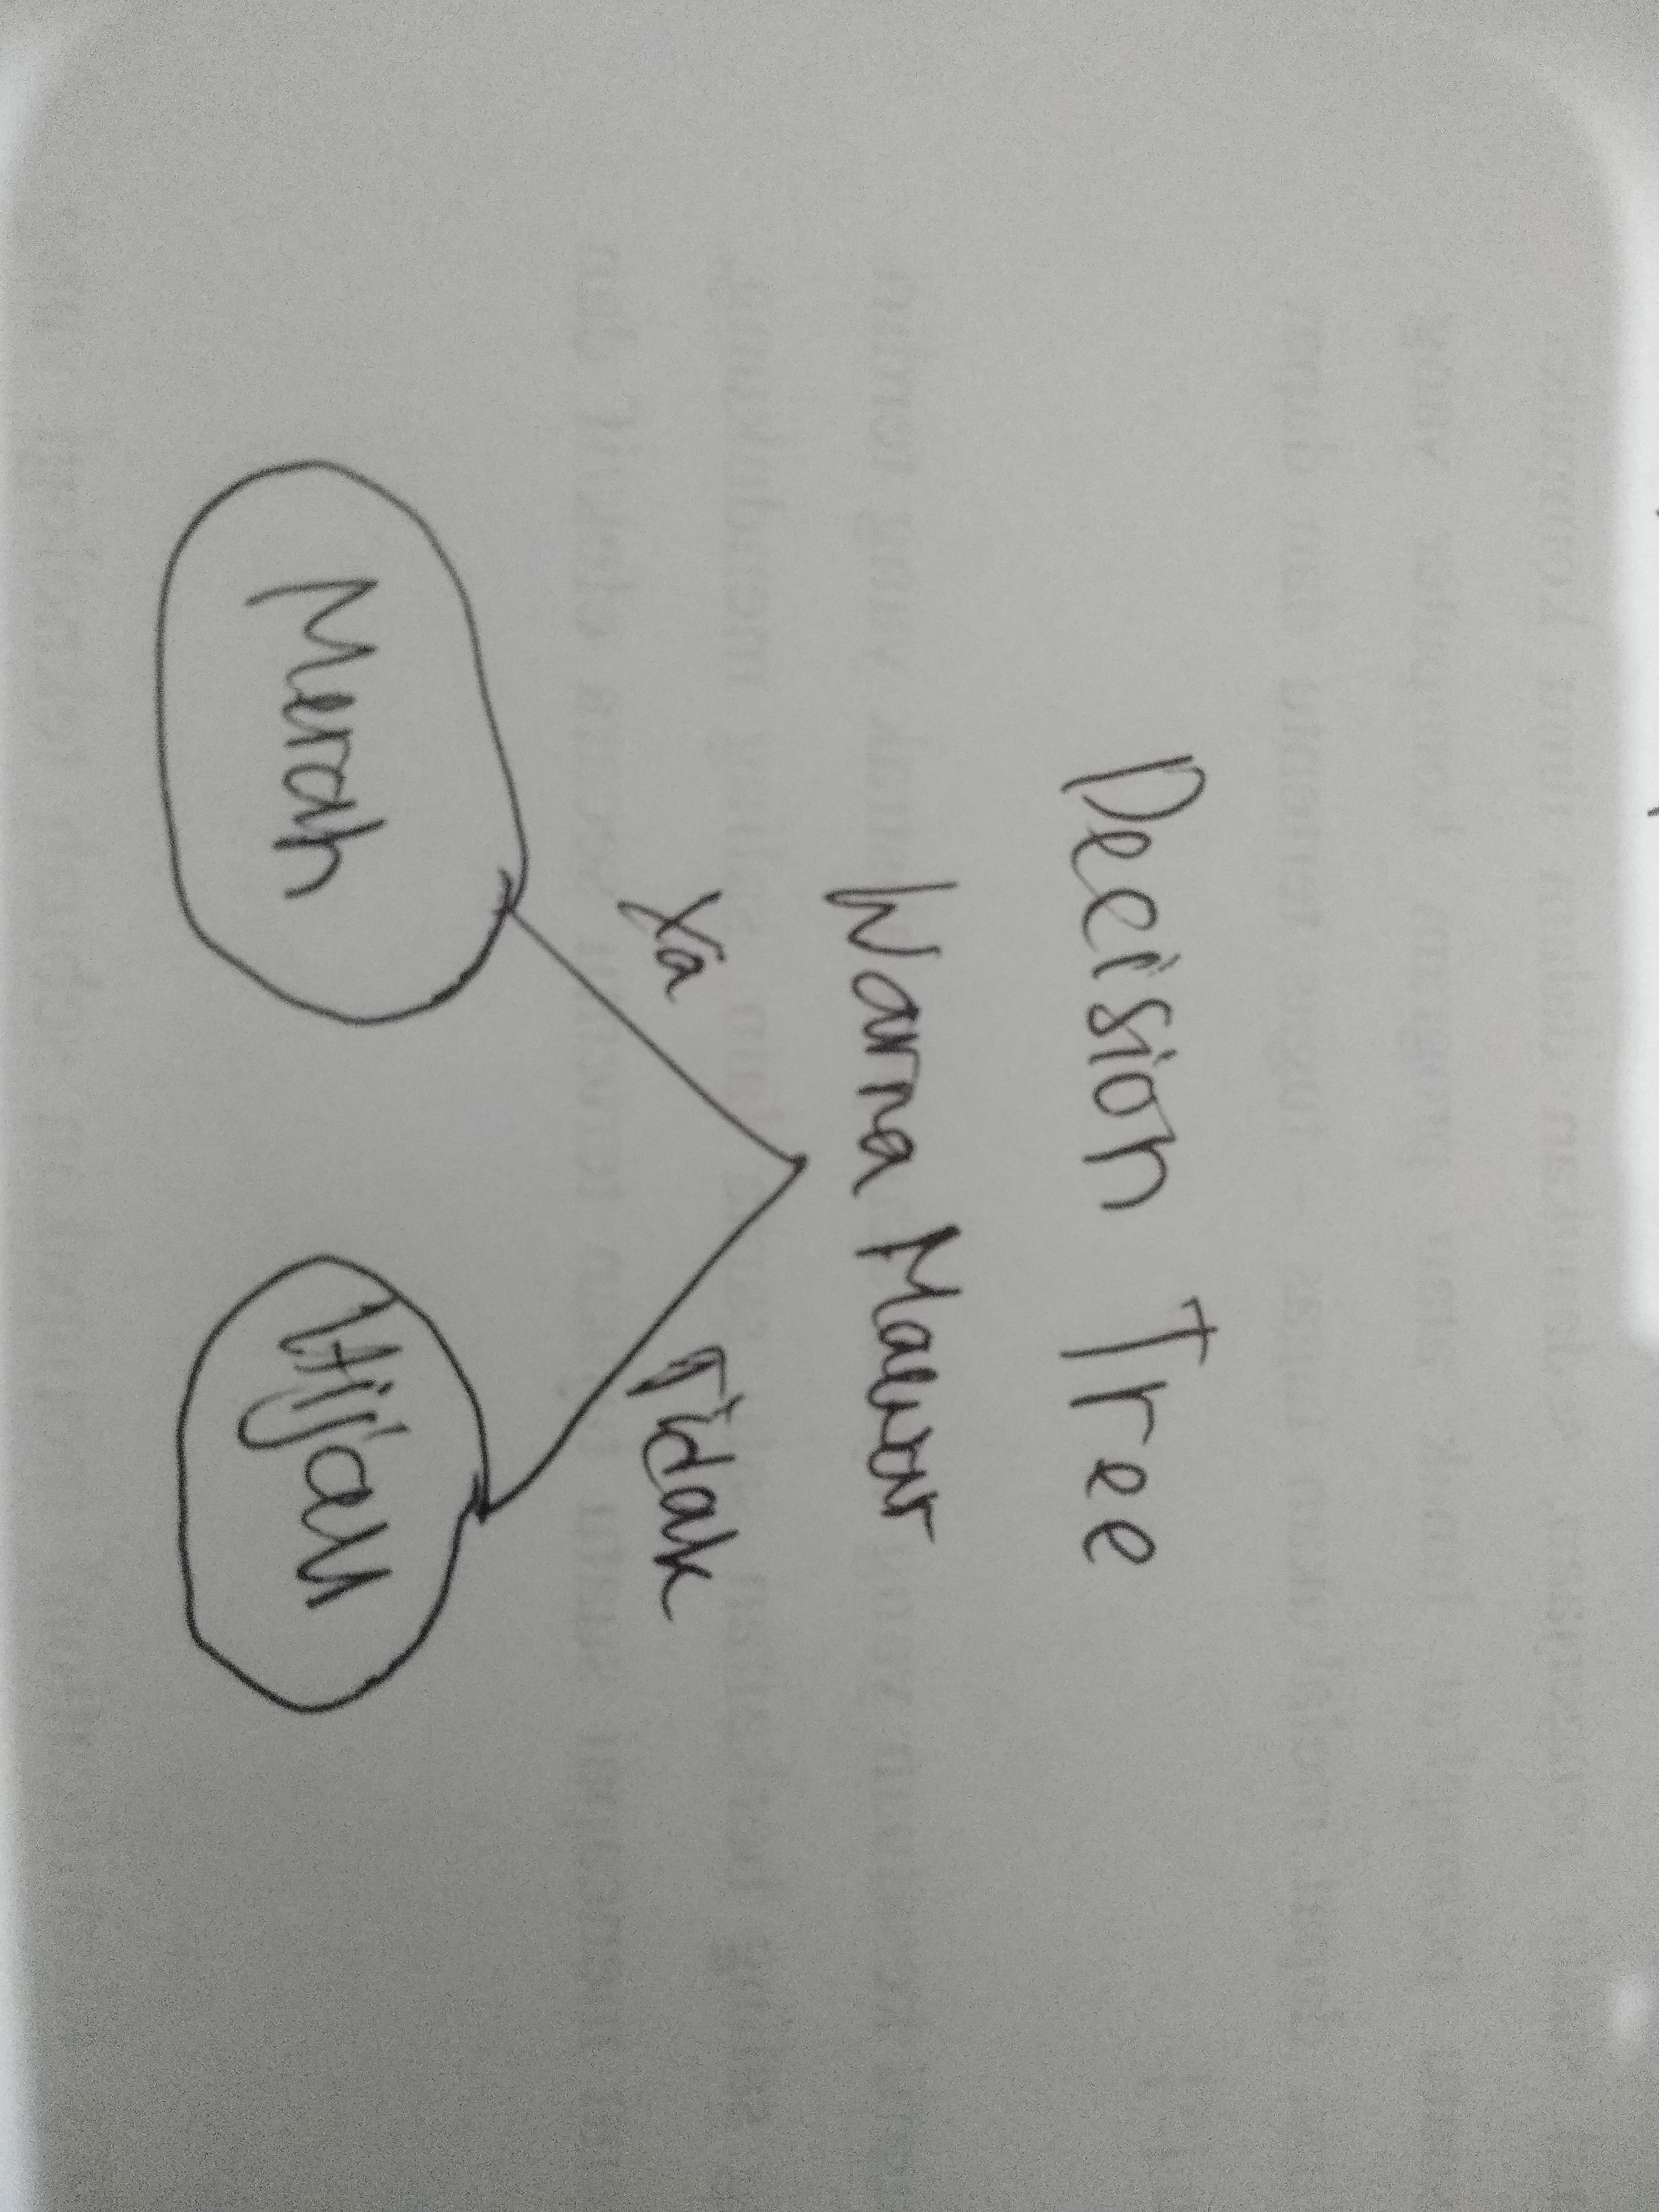
\includegraphics[scale=0.5]{figures/1174057/chapter3/8.PNG}
\caption{hasil}
\label{contoh4}
\end{figure}

\item Confusion Matrix\par
arti codingan pada hasil tiap codingan confusion matrix pada baris pertama codingan tersebut mendeskripsikan atau mengimport confusion matrix dari sklearn kemudian dibuat variabel y\_true untuk nilai target ground truth (benar). y\_pred untuk Taksiran target seperti yang dikembalikan oleh classifier. lalu menampilkan kedua variabel. hasil pada gambar \ref{contoh5} .
\lstinputlisting{src/1174057/chapter3/6.py}
\begin{figure}[ht]
\centering
\includegraphics[scale=0.5]{figures/1174057/chapter3/9.PNG}
\caption{hasil}
\label{contoh5}
\end{figure}

\item SVM dan Decision Tree\par
Seperti pengklasifikasi lainnya, DecisionTreeClassifier mengambil input dua array: array X, jarang atau padat, dengan ukuran n\_samples, n\_features memegang sampel pelatihan, dan array Y dari nilai integer, ukuran n\_samples,Atau, probabilitas setiap kelas dapat diprediksi. Seperti pengklasifikasi lainnya, SVC, NuSVC dan LinearSVC mengambil input dua array: array X ukuran n\_samples, n\_features memegang sampel pelatihan, dan array y label kelas (string atau bilangan bulat), ukuran n\_samples:. hasil pada gambar \ref{contoh6} .
\lstinputlisting{src/1174057/chapter3/7.py}
\begin{figure}[ht]
\centering
\includegraphics[scale=1]{figures/1174057/chapter3/10.PNG}
\caption{hasil}
\label{contoh6}
\end{figure}

\item Cross Validation\par
 digunakan untuk memeriksa akurasi dari ketepatan hasil pengolahan data tersebut maka akan didapat nilai rata-rata 60 persen dari hasil pengolahan data tersebut untuk lebih jelasnya dapat di lihat pada gambar pada codingan tersebut pada baris ke satu melakukan import library dari sklern kemudian pada baris selanjutnya mengisi nilai skor dengan nilai pada variabel lontong setelah hal tersebut dilakukan kemudian data tersebut di eksekusi. berikut merupakan hasil dari code tersebut dapat dilihat pada gambar \ref{contoh7} .
\lstinputlisting{src/1174057/chapter3/8.py}
\begin{figure}[ht]
\centering
\includegraphics[scale=1]{figures/1174057/chapter3/11.PNG}
\caption{hasil}
\label{contoh7}
\end{figure}

\item program pengamatan
arti dari hasil program pengamatan. perogram pengamatan dapat mengamati dari 3 aspek diatas yaitu svm, random, dan decision tree. Yang memiliki variabel X Y Z dan di tampilkan dalam bentuk grafik pada gambar \ref{contoh8}. 
\lstinputlisting{src/1174057/chapter3/9.py}
\begin{figure}[ht]
\centering
\includegraphics[scale=1]{figures/1174057/chapter3/12.PNG}
\caption{hasil}
\label{contoh8}
\end{figure}
\end{enumerate}


\subsection{Penanganan Error}
Screenshot error
\begin{enumerate}
\item  Gambar error
\begin{figure}[ht]
\centering
\includegraphics[scale=1]{figures/1174057/chapter3/error.PNG}
\caption{hasil}
\label{error}
\end{figure}
\end{enumerate}

Code Errornya 
\begin{verbatim}
import pandas as alit
cewek = {"List Nama Cewek Alit" : ['Triya','Mirla','Alit','Merita']}
af = alit.DataFrame(cewek)
print('Alit sayang + af)
\end{verbatim}
\par
pada bagian print, perintah ketika akan menjalankan program. terdapat kesalahan pada tanda petik yang kurang sehingga program tidak dapat dijalankan. 

\par perbaiki code error
\begin{verbatim}
import pandas as alit
cewek = {"List Nama Cewek Alit" : ['Triya','Mirla','Alit','Merita']}
af = alit.DataFrame(cewek)
print('Alit sayang ' + af)
\end{verbatim}

